\section{Introduction}
%Each section needs a subsection for the small points on top to show up
\subsection{Dummy}

\begin{frame}{A quasiperiodic puzzle [Bédaride \etal{} 12]}

\centering
\includegraphics[width=.5\textwidth]{img/1_intro/tiles_euro.pdf}

Pay the squares, get the rhombuses for free!

\(
\<{6cm}
\centering
\includegraphics[width=.8\textwidth]{img/1_intro/forbidden.pdf}

Forbidden configuration.
\>

\<{6cm}
\centering
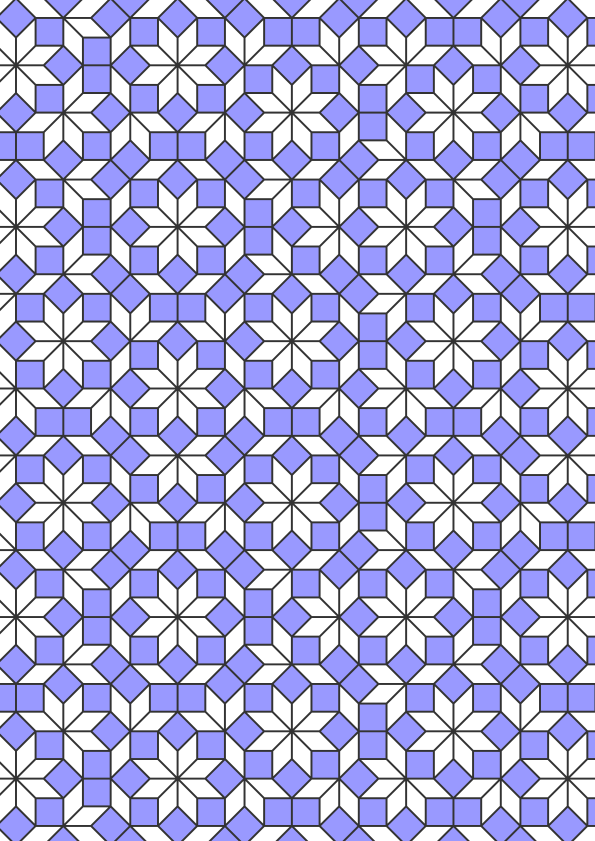
\includegraphics[width=1.\textwidth]{img/1_intro/ammann.pdf}

Patch of the Ammann-Beenker tiling.
\>
\)
\end{frame}

\begin{frame}{Periodic, quasiperiodic and random}
\centering
\only<2>{
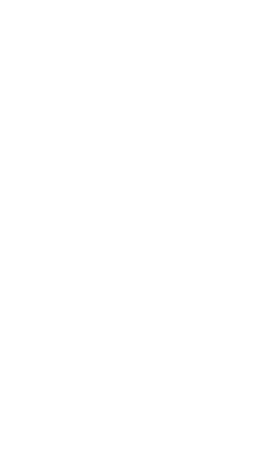
\includegraphics[width=.6\textwidth]{img/1_intro/periodic.pdf}

periodic}

\only<3>{
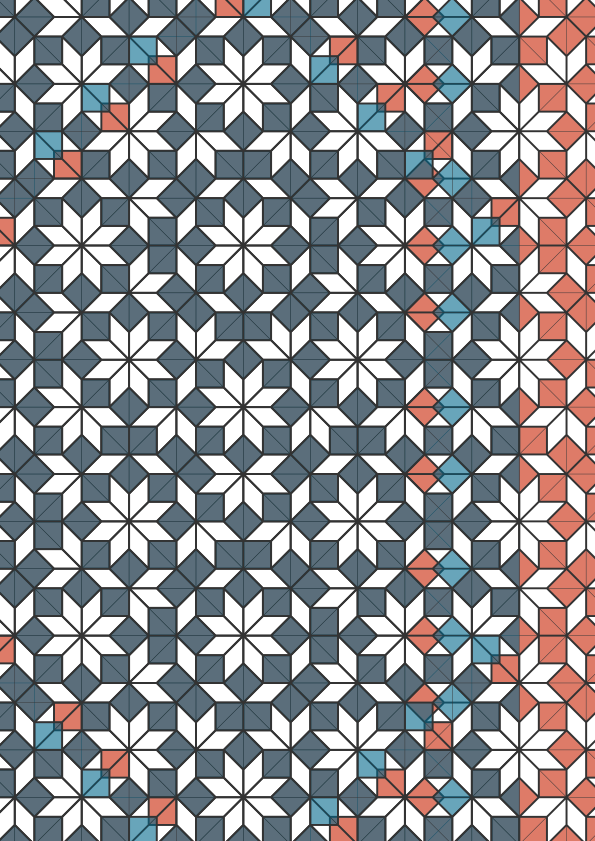
\includegraphics[width=.6\textwidth]{img/1_intro/quasiperiodic.pdf}

quasiperiodic 

\flushleft{(Meyer sets, see eg [Grimm, Baake 13])}
}

\only<1>{
\centering
\includegraphics[width=.6\textwidth]{img/1_intro/random.pdf}

random}
\end{frame}

\begin{frame}{From tiles to atoms}
\centering
\includegraphics[width=.6\textwidth]{img/1_intro/AB_tiling_and_plot.pdf}

$\rightarrow$ can atoms arrange in a quasiperiodic fashion?
\end{frame}

\begin{frame}{Quasicrystals}
A quasicrystal is:
\begin{itemize}
	\item \textbf{aperiodic}
	\item \textbf{long range ordered} (its diffraction pattern exhibits sharp peaks).
\end{itemize}
%\textbf{Aperiodic tilings} are used to model quasicrystals.
\(
	\<{6cm}
		\centering
		\includegraphics[scale=0.1]{img/1_intro/diffraction_tenfold.png}
		
		\ss{Diffraction pattern of a AlPdMn alloy} \ss{(Conradin Beeli group)}
	\>
	\<{6cm}
		\centering
		\includegraphics[scale=0.06]{img/1_intro/penrose.png}
		
		\ss{A patch of the quasiperiodic Penrose tiling,} \ss{used to model many quasicrystals.}
	\>
\)
\end{frame}

\begin{frame}{Examples of quasicrystals}
\(
	\<{6cm}
		\centering
		\includegraphics[scale=0.28]{img/1_intro/homgzn.png}
		
		\ss{HoMgZn alloy in its icosahedral phase} \ss{(\url{doi:10.1038/nmat1244})}
	\>
	\<{6cm}
		\centering
		\includegraphics[scale=0.22]{img/1_intro/wasio.jpg}
		
		\ss{A 2D molecular quasicrystal} \ss{(\url{doi:10.1038/nature12993})}
	\>
\)

\begin{itemize}
	\item many intermetallic alloys are quasiperiodic
	\item a single natural example: Khatyrka meteorite hosts quasicrystals \ss{(\url{doi:10.1126/science.1170827})}. 
\end{itemize}
\end{frame}
